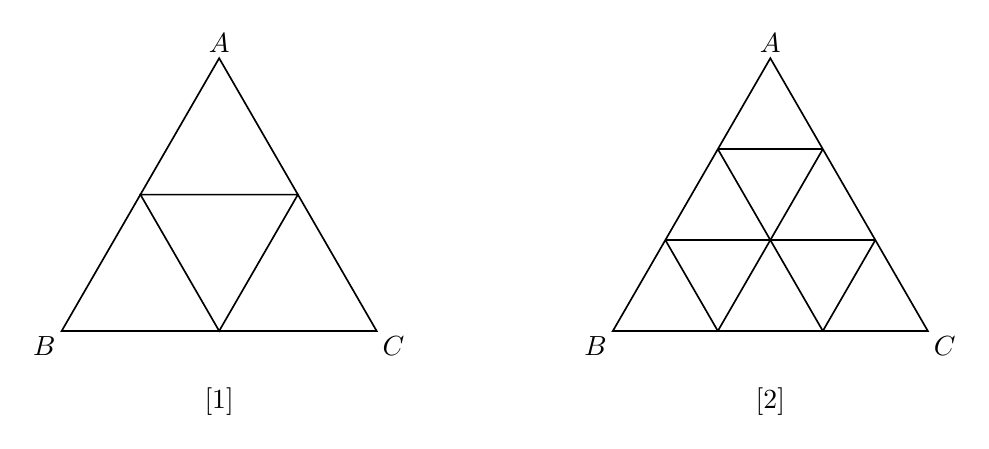
\begin{tikzpicture}[x=1cm,y=1cm,font=\normalsize,
 geometry edge/.style={solid,line width=.6pt},
 geometry mark/.style={solid,line width=.6pt},
 geometry label/.style={font=\normalsize,inner sep=2pt}]
\coordinate (F1A) at (2.0,3.4641);
\coordinate (F1B) at (0.0,0.0);
\coordinate (F1C) at (4.0,0.0);
\coordinate (F1AB) at (1.0,1.7321);
\coordinate (F1AC) at (3.0,1.7321);
\coordinate (F1BC) at (2.0,0.0);
\coordinate (F2A) at (9.0,3.4641);
\coordinate (F2B) at (7.0,0.0);
\coordinate (F2C) at (11.0,0.0);
\coordinate (F2AB1) at (8.3333,2.3094);
\coordinate (F2AB2) at (7.6667,1.1547);
\coordinate (F2AC1) at (9.6667,2.3094);
\coordinate (F2AC2) at (10.3333,1.1547);
\coordinate (F2BC1) at (8.3333,0.0);
\coordinate (F2BC2) at (9.6667,0.0);
\coordinate (F2CTR) at (9.0,1.1547);
\coordinate (F1CAP) at (2.0,-0.9);
\coordinate (F2CAP) at (9.0,-0.9);
\draw[geometry edge] (F1A)--(F1AB)--(F1B)--(F1BC)--(F1C)--(F1AC)--cycle;
\draw[geometry edge] (F1AB)--(F1AC)--(F1BC)--cycle;
\draw[geometry edge] (F2A)--(F2AB1)--(F2AB2)--(F2B)--(F2BC1)--(F2BC2)--(F2C)--(F2AC2)--(F2AC1)--cycle;
\draw[geometry edge] (F2AB1)--(F2AC1);
\draw[geometry edge] (F2AB2)--(F2CTR)--(F2AC2);
\draw[geometry edge] (F2AC1)--(F2CTR)--(F2BC1);
\draw[geometry edge] (F2AB1)--(F2CTR)--(F2BC2);
\draw[geometry edge] (F2AB2)--(F2BC1);
\draw[geometry edge] (F2AC2)--(F2BC2);
\node[geometry label,above] at (F1A) {$A$};
\node[geometry label,below left] at (F1B) {$B$};
\node[geometry label,below right] at (F1C) {$C$};
\node[geometry label,above] at (F2A) {$A$};
\node[geometry label,below left] at (F2B) {$B$};
\node[geometry label,below right] at (F2C) {$C$};
\node[font=\normalsize,inner sep=2pt] at (2.0,-0.9) {\bitmapinsertcaption[1]};
\node[font=\normalsize,inner sep=2pt] at (9.0,-0.9) {\bitmapinsertcaption[2]};
\end{tikzpicture}
